\documentclass[11pt]{article}
\usepackage[margin=1in]{geometry}
\usepackage[T1]{fontenc}
\usepackage[utf8]{inputenc}
\usepackage{lmodern}
\usepackage{amsmath}
\usepackage{graphicx}
\usepackage{booktabs}
\usepackage[hidelinks]{hyperref}
\usepackage{microtype}
\usepackage[font=small,labelfont=bf]{caption}

% generated by paper/make_numbers.py from results/ -- do not edit
\newcommand{\Neurons}{384}
\newcommand{\Inputs}{314}
\newcommand{\NLPLCtwo}{210}
\newcommand{\NLCfour}{104}
\newcommand{\Intermediates}{60}
\newcommand{\Outputs}{10}
\newcommand{\Edges}{5810}
\newcommand{\ExcPct}{90.6}
\newcommand{\NAch}{5264}
\newcommand{\NGaba}{443}
\newcommand{\NGlut}{103}
\newcommand{\NParams}{64}
\newcommand{\NSeeds}{5}
\newcommand{\TestGames}{200}
\newcommand{\BudgetFrames}{1{,}000{,}000}
\newcommand{\MeanPipesAll}{100.0}
\newcommand{\WinRateAll}{100}
\newcommand{\GensMin}{8}
\newcommand{\GensMax}{11}
\newcommand{\TrainTimeMean}{50}
\newcommand{\TrainTimeMax}{55}
\newcommand{\HeurMean}{84.2}
\newcommand{\HeurWin}{68}
\newcommand{\RandMean}{0.07}
\newcommand{\EdgesDirect}{804}
\newcommand{\EdgesInMid}{2540}
\newcommand{\EdgesMidOut}{215}
\newcommand{\LesBrokenCount}{3}
\newcommand{\LesConditions}{8}
\newcommand{\LesionRows}{intact & 100.0 & 100.0 & 100.0 & 100.0 & 100.0 \\ all intermediates & 100.0 & 100.0 & 100.0 & 100.0 & 100.0 \\ LC4 inputs & 100.0 & 100.0 & 100.0 & 100.0 & 100.0 \\ LPLC2 inputs & 100.0 & 100.0 & 100.0 & 3.7 & 100.0 \\ DNp01 output & 100.0 & 7.5 & 100.0 & 100.0 & 100.0 \\ DNp02 output & 100.0 & 100.0 & 100.0 & 100.0 & 100.0 \\ DNp04 output & 100.0 & 100.0 & 100.0 & 2.5 & 100.0 \\ DNp06 output & 100.0 & 100.0 & 100.0 & 100.0 & 100.0 \\ DNp11 output & 100.0 & 100.0 & 100.0 & 100.0 & 100.0 \\}


\title{\textbf{Flapping on Command: a \textit{Drosophila} Escape Pathway\\as the Controller of a Flappy Bird Agent}}
\author{Burak G\"ulmez\\[2pt]
\small College of Engineering and Architecture, University College Dublin, Dublin, Ireland\\
\small \texttt{burak.gulmez@ucd.ie}}
\date{}

\begin{document}
\maketitle

\begin{abstract}
\noindent
Escape in flies is triggered by a compact pathway in which looming-sensitive visual neurons converge
on a small set of descending neurons. That pathway is extracted here from the FlyWire adult brain
reconstruction (\Neurons{} neurons, \Edges{} connections), its weights are frozen, and it is used as
the controller of a Flappy Bird agent. Only \NParams{} interface numbers are optimised by an
evolution strategy; each run converges in \GensMin{}--\GensMax{} generations and about
\TrainTimeMean{}\,s on a laptop CPU. In all \NSeeds{} runs the maximum of 100 pipes is cleared in
every one of \TestGames{} unseen courses, whereas \HeurMean{} pipes are cleared on average by a tuned
hand-written rule. Silencing experiments show why the task is easier than it looks: the input neurons
contact the output neurons directly, so behaviour is unaffected when all \Intermediates{}
intermediate neurons are removed, while individual runs come to depend on different single cell
types. The study is a reproducible demonstration, not a model of escape behaviour.
\end{abstract}

\textbf{Keywords:} connectome; escape pathway; giant fiber; neuroevolution; closed-loop control

\section{Introduction}
The adult fly connectome released by the FlyWire consortium \cite{dorkenwald2024}, together with a
parts list and wiring diagram of the visual system \cite{matsliah2024} and neurotransmitter
predictions obtained from the electron-microscopy images \cite{eckstein2024}, makes small,
behaviourally meaningful circuits easy to isolate. One of the best characterised is the
looming-escape pathway. LPLC2 neurons were described as ultra-selective looming detectors whose
selectivity arises from radial motion opponency \cite{klapoetke2017}. In the giant fiber escape
circuit, one visual input type was found to encode angular expansion velocity and another angular
size, and motor program selection and timing were shown to emerge from the linear integration of
these two features within the giant fiber \cite{vonreyn2017}.

Simulation of connectome circuits at the level of activity is becoming routine: a leaky
integrate-and-fire model of the whole fly brain, built from connectivity and transmitter identity,
predicted which neurons respond to tastes and which are required for feeding initiation
\cite{shiu2024}. A closed sensorimotor loop, in which the output of the circuit changes the stimuli it
receives next, is rarely included in such models. That loop is closed here with the simplest possible
one-button task. Flappy Bird is a natural match for an escape circuit, because the only decision is
when to trigger an upward impulse. The game has also been used to compare agents obtained by
evolutionary search and by deep reinforcement learning \cite{thurler2021}.

Methodologically, the network is a fixed recurrent circuit with trained input and output maps, an
arrangement studied for generic recurrent circuits under the name of liquid state machines
\cite{maass2002}. The interface is optimised with CMA-ES \cite{hansen2001}. Evolution strategies of
this kind have been proposed as a scalable, easily parallelised alternative to reinforcement learning
\cite{salimans2017}, which suits small controllers evaluated on CPUs.

Three things are provided: a minimal, fully seeded pipeline from the connectome tables to a playing
agent; a quantitative report over independent runs and reference agents; and a silencing analysis
that identifies which part of the circuit is actually used by the learned solutions.

\section{Methods}

\paragraph{Circuit.}
From the FlyWire v783 tables, LPLC2 (\NLPLCtwo{} cells) and LC4 (\NLCfour{}) were taken as inputs and
the descending neurons DNp01 (the giant fiber), DNp02, DNp04, DNp06 and DNp11 (two each) as outputs.
Any further neuron receiving at least 40 synapses in total from the inputs and sending at least 40 to
the outputs was kept as an intermediate (\Intermediates{} cells). This gave \Neurons{} neurons and
\Edges{} connections of at least five synapses. Weights were set to $\pm\log(1+\text{synapses})$ with
signs from predicted transmitters \cite{eckstein2024}: \NAch{} cholinergic connections positive,
\NGaba{} GABAergic and \NGlut{} glutamatergic negative, so that \ExcPct\% of connections are
excitatory. The weight matrix was scaled to spectral radius $0.9$. Of the connections,
\EdgesDirect{} run directly from inputs to outputs, \EdgesInMid{} from inputs to intermediates and
\EdgesMidOut{} from intermediates to outputs (Fig.~\ref{fig:circuit}).

\paragraph{Task.}
In a unit-height world the bird is placed at $x=0.25$ with radius $0.025$. Per frame, $0.002$ is
subtracted from the vertical velocity (fall speed capped at $0.04$), and a flap sets the velocity to
$+0.02$. Pipes are $0.10$ wide, spaced $0.55$ apart and moved left by $0.01$ per frame; their gaps
are $0.30$ high, with centres drawn uniformly from $[0.25,0.75]$ by a seeded xorshift generator. A
run ends on contact with the floor, the ceiling or a pipe, and is won after 100 pipes. These
constants were fixed before any network was trained, such that the reference rule below plays well.

\paragraph{Network and training.}
Six readings per frame (height, vertical velocity, horizontal distance to the next pipe, and the gap
centre, top and bottom relative to the bird) are mapped onto eight input groups by a trained linear
map. States follow $x \leftarrow x + a(-x + g\,W\tanh(x) + I)$ with four updates per frame. The mean
$\tanh$ activity of each output cell type enters a trained weighted sum, and a flap is issued when
the sum is positive. The trained parameters are the input map and biases, five readout weights, one
bias, the leak and the gain, \NParams{} in total. CMA-ES \cite{hansen2001} was run with population 16
and eight courses per candidate until \BudgetFrames{} frames had been simulated. Disjoint seeds were
used for training, validation and test courses, and the procedure was repeated for \NSeeds{} seeds.

\paragraph{References and silencing.}
Two reference agents were evaluated on the same test courses: a rule that flaps when the height
predicted three frames ahead falls below the gap centre minus $0.08$, and an agent that flaps in a
random 10\% of frames. For the lesion analysis, the $\tanh$ output of a group of neurons was forced
to zero and the test courses were replayed.

\begin{figure}[t]
\centering
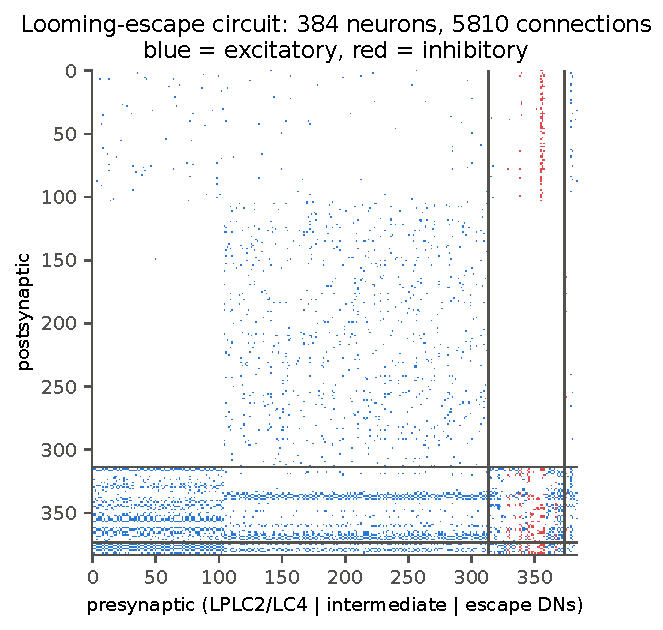
\includegraphics[width=0.40\linewidth]{../figures/fig1_circuit.pdf}\hfill
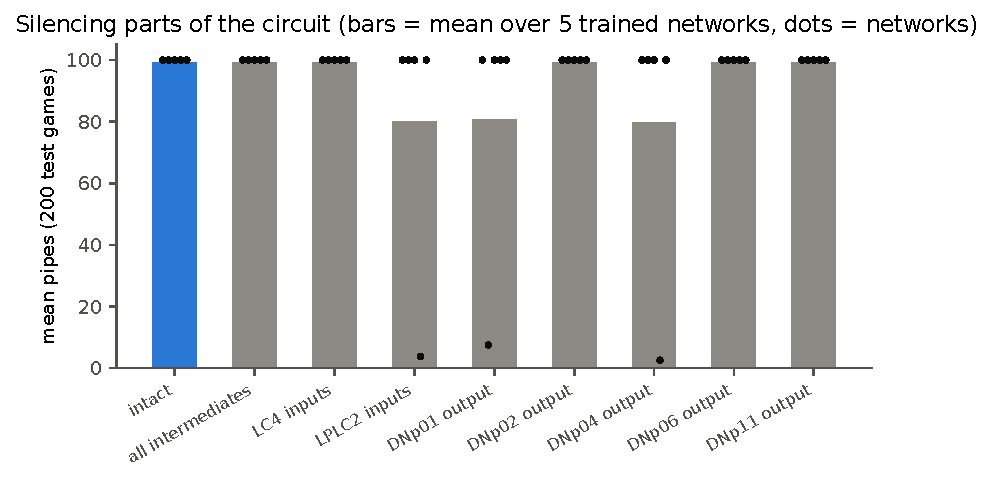
\includegraphics[width=0.57\linewidth]{../figures/fig4_lesion.pdf}
\caption{Left: the extracted escape pathway (inputs, intermediates, outputs; blue excitatory, red
inhibitory). Right: mean pipes cleared after silencing a group of neurons; dots are the five trained
networks.}
\label{fig:circuit}
\end{figure}

\section{Results}
In every trained network, 100 of 100 pipes were cleared in all \TestGames{} test courses
(mean \MeanPipesAll{}, \WinRateAll\% wins), after \GensMin{}--\GensMax{} generations and at most
\TrainTimeMax{}\,s of optimisation. On the same courses, \HeurMean{} pipes were cleared by the
hand-written rule (\HeurWin\% complete runs) and \RandMean{} by random flapping. The behaviour
consists of a steady sequence of short flaps interleaved with glides, with longer climbs when
consecutive gaps differ in height (Fig.~\ref{fig:traj}).

The ease of the task is explained by the silencing results. Nothing changed in any of the five
networks when all \Intermediates{} intermediate neurons were removed, which is possible because the
inputs and outputs are bridged by \EdgesDirect{} direct connections. Most single-group silencings
were equally harmless: a network dropped below 50 pipes in only \LesBrokenCount{} of the
$5\times\LesConditions{}$ conditions. Those few cases are informative because they differ across
runs: one network collapsed without the giant fiber DNp01, another without LPLC2 or without DNp04.
Different routes through the same frozen circuit were therefore found by independent optimisations.

\begin{figure}[t]
\centering
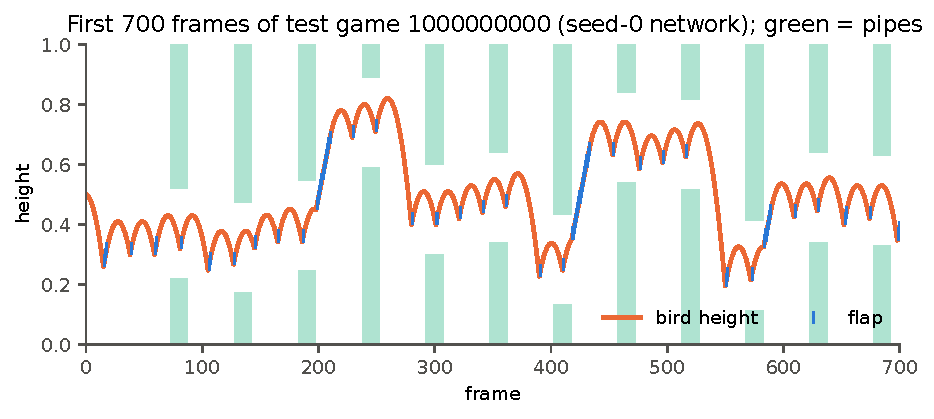
\includegraphics[width=0.95\linewidth]{../figures/fig3_trajectory.pdf}
\caption{Height and flap times over the first 700 frames of a test course; green bands are pipes.}
\label{fig:traj}
\end{figure}

\section{Discussion}
A frozen escape pathway plus \NParams{} trained numbers is sufficient to play this game perfectly,
which is mainly a statement about the task: the gap is already localised by the six readings, and the
game is played reasonably well by a two-condition rule. Matched random graphs were not evaluated in
this study, so no advantage of the measured wiring is claimed. The comparison that is reported,
between parts of the circuit, shows that the short direct route is preferred by the learned solutions
and that the loss of the multisynaptic route is tolerated. Biologically the model is deliberately
thin: rate units are used instead of spiking neurons, synapse counts serve as weights, transmitter
identities are predicted rather than measured, and neither optic-lobe preprocessing nor a body is
included. Flies also do not flap through pipes; the analogy between triggering an escape and
triggering a flap guided the choice of circuit and nothing more. A natural extension would be to
drive the same pathway with rendered looming stimuli instead of abstract readings.

\section{Conclusion}
The looming-escape pathway of \textit{Drosophila}, taken from FlyWire and left unchanged, controls a
Flappy Bird agent by which every test course is completed after about a minute of CPU training.

\paragraph{Data and code availability.} The connectome tables (FlyWire v783) are obtained from the
FlyWire Codex portal \cite{dorkenwald2024}. Scripts, configuration files, raw logs and the JavaScript
re-implementation used by the demo can be found at
\url{https://github.com/burakgulmez/fly-flappybird}.

\bibliographystyle{plain}
\bibliography{refs}
\end{document}
